\documentclass[10pt,sigconf]{acmart}

\usepackage{booktabs} % For formal tables
\usepackage{xspace}
\usepackage{subfigure}
\usepackage{graphicx}

% Copyright
%\setcopyright{none}
%\setcopyright{acmcopyright}
%\setcopyright{acmlicensed}
\setcopyright{rightsretained}
%\setcopyright{usgov}
%\setcopyright{usgovmixed}
%\setcopyright{cagov}
%\setcopyright{cagovmixed}


% DOI
%\acmDOI{10.475/123_4}

% ISBN
%\acmISBN{123-4567-24-567/08/06}

%Conference
%\acmConference[WOODSTOCK'97]{ACM Woodstock conference}{July 1997}{El Paso, Texas USA}
%\acmYear{1997}
%\copyrightyear{2016}

%\acmArticle{4}

% These commands are optional
%\acmBooktitle{Transactions of the ACM Woodstock conference}
%\editor{Jennifer B. Sartor}
%\editor{Theo D'Hondt}
%\editor{Wolfgang De Meuter}

\copyrightyear{2018}
\acmYear{2018}
\acmConference[MobiCom '18]{The 24th Annual International Conference on Mobile Computing and Networking}{October 29-November 2, 2018}{New Delhi, India}
\acmBooktitle{The 24th Annual International Conference on Mobile Computing and Networking (MobiCom '18), October 29-November 2, 2018, New Delhi, India}
\acmDOI{10.1145/3241539.3267755}
\acmISBN{978-1-4503-5903-0/18/10}
\acmPrice{}

\begin{document}
\fancyhead{}
\newcommand{\name}{\emph{AMuSe}\xspace}

\title{Poster: \name: An \underline{A}gile \underline{Mu}ltipath TCP \underline{S}ch\underline{e}duler for Dual-Band 802.11ad/ac Wireless LANs}
%\titlenote{Produces the permission block, and copyright information}
%\subtitle{Extended Abstract}
%\subtitlenote{The full version of the author's guide is available as \texttt{acmart.pdf} document}

\author{Swetank Kumar Saha$^1$, Shivang Aggarwal$^1$, Dimitrios Koutsonikolas$^1$, Joerg Widmer$^2$}
%\authornote{Dr.~Trovato insisted his name be first.}
%\orcid{1234-5678-9012}
\affiliation{%
  \institution{$^1$University at Buffalo, The State University of New York, $^2$IMDEA Neworks Institute, Madrid, Spain}
  %\streetaddress{P.O. Box 1212}
  %\city{Dublin}
  %\state{Ohio}
  %\postcode{43017-6221}
}
\email{{swetankk,shivanga,dimitrio}@buffalo.edu,joerg.widmer@imdea.org}

\begin{comment}
\author{Lars Th{\o}rv{\"a}ld}
\authornote{This author is the
  one who did all the really hard work.}
\affiliation{%
  \institution{The Th{\o}rv{\"a}ld Group}
  \streetaddress{1 Th{\o}rv{\"a}ld Circle}
  \city{Hekla}
  \country{Iceland}}
\email{larst@affiliation.org}

\author{Valerie B\'eranger}
\affiliation{%
  \institution{Inria Paris-Rocquencourt}
  \city{Rocquencourt}
  \country{France}
}
\author{Aparna Patel}
\affiliation{%
 \institution{Rajiv Gandhi University}
 \streetaddress{Rono-Hills}
 \city{Doimukh}
 \state{Arunachal Pradesh}
 \country{India}}
\author{Huifen Chan}
\affiliation{%
  \institution{Tsinghua University}
  \streetaddress{30 Shuangqing Rd}
  \city{Haidian Qu}
  \state{Beijing Shi}
  \country{China}
}

\author{Charles Palmer}
\affiliation{%
  \institution{Palmer Research Laboratories}
  \streetaddress{8600 Datapoint Drive}
  \city{San Antonio}
  \state{Texas}
  \postcode{78229}}
\email{cpalmer@prl.com}

\author{John Smith}
\affiliation{\institution{The Th{\o}rv{\"a}ld Group}}
\email{jsmith@affiliation.org}

\author{Julius P.~Kumquat}
\affiliation{\institution{The Kumquat Consortium}}
\email{jpkumquat@consortium.net}
\end{comment}

% The default list of authors is too long for headers.
\renewcommand{\shortauthors}{B. Trovato et al.}
%\renewcommand\footnotetextcopyrightpermission[1]{}

\begin{abstract}
\if 0 % old abstract
Utilizing 2.16 GHz wide channels, 802.11ad links can provide data rates
up to 6.7 Gbps but remain highly susceptible to blockage and
disconnection due to mobility. Legacy 802.11ac/n links, on the other
hand, provide much lower rates but are robust even under dynamic
scenarios. In this work, we explore using Multipath TCP (MPTCP) to
engage both 802.11ad and 802.11ac interfaces simultaneously for
performance speed-up and improved reliability through seamless
switching. Our measurements show that vanilla MPTCP can achieve these
goals only under static conditions but may often result in performance
worse than the faster of the two interfaces under many dynamic
scenarios. We implement a new MPTCP scheduler \name to 
%address such cases and 
allow MPTCP to perform near-optimally under all
scenarios. Our evaluation shows that \name can boost performance by up
to 2.5x and accelerate traffic stream re-establishment by 10s of
seconds.
\fi

802.11ad links provide data rates up to 6.7 Gbps but remain highly
susceptible to blockage and mobility. On the other hand, legacy
802.11ac/n links yield much lower rates but are robust even under
dynamic scenarios. In this work, we explore using Multipath TCP
(MPTCP) to engage both 802.11ad and 802.11ac interfaces simultaneously
for performance speed-up and improved reliability. We show that
vanilla MPTCP achieves these goals under static conditions but often
results in performance worse than using the faster interface alone
under dynamic scenarios. We then design and implement \name, a new
MPTCP scheduler that allows MPTCP to perform near-optimally under all
scenarios.
\end{abstract}

\begin{comment}%
% The code below should be generated by the tool at
% http://dl.acm.org/ccs.cfm
% Please copy and paste the code instead of the example below.
%
\begin{CCSXML}
<ccs2012>
 <concept>
  <concept_id>10010520.10010553.10010562</concept_id>
  <concept_desc>Computer systems organization~Embedded systems</concept_desc>
  <concept_significance>500</concept_significance>
 </concept>
 <concept>
  <concept_id>10010520.10010575.10010755</concept_id>
  <concept_desc>Computer systems organization~Redundancy</concept_desc>
  <concept_significance>300</concept_significance>
 </concept>
 <concept>
  <concept_id>10010520.10010553.10010554</concept_id>
  <concept_desc>Computer systems organization~Robotics</concept_desc>
  <concept_significance>100</concept_significance>
 </concept>
 <concept>
  <concept_id>10003033.10003083.10003095</concept_id>
  <concept_desc>Networks~Network reliability</concept_desc>
  <concept_significance>100</concept_significance>
 </concept>
</ccs2012>
\end{CCSXML}

\ccsdesc[500]{Computer systems organization~Embedded systems}
\ccsdesc[300]{Computer systems organization~Redundancy}
\ccsdesc{Computer systems organization~Robotics}
\ccsdesc[100]{Networks~Network reliability}


\keywords{ACM proceedings, \LaTeX, text tagging}
\end{comment}

\maketitle

\graphicspath{{figs/}}

\section{Introduction}
Millimeter-wave (mmWave) wireless is fast emerging as the prime
candidate technology for providing multi-Gbps data rates in future wireless networks.
%, WLANs and for fixed wireless access.
% Although
%different parts of the mmWave spectrum (both licensed and unlicensed)
%are currently being explored by the industry, 
The IEEE 802.11ad
standard 
%and its successor 802.11ay specifically target indoor
%WLANs. 802.11ad 
%utilizes the almost 7 GHz of unlicensed spectrum
%centered around 60 GHz to 
provides data rates of up to 6.7 Gbps. 
It
achieves this multi-fold increase over legacy WiFi through
2 GHz-wide channels.
%ization (2.16 GHz, 13.5x wider compared to the 160
%MHz of 802.11ac) and directional antennas.
%Multiple commercial devices (both APs and laptops) supporting the standard have been
%released over the past few years. 
%and the technology is already making
%its way into smartphones. ~\cite{peraso_802.11ad,asus_802.11ad}.
Nonetheless, communication at mmWave frequencies faces fundamental
challenges due to the high propagation and penetration loss. %Although 
The use of directional transmissions 
%overcomes the severe attenuation, it 
makes
links susceptible to disruption by human blockage and client
mobility. 
%While several recent works have explored ways of dealing with blockage and mobility, e.g., by
%proposing efficient beamsteering techniques, link outages remain a
%major challenge preventing 802.11ad from providing the seamless
%connectivity that legacy WiFi does. 
Even if future PHY/MAC improvements may result in faster beam steering, any realistic
indoor scenario is expected to contain enough dynamism
%, in terms of
%environmental and device mobility, 
to cause a large number of re-connection events.
% which will hurt application performance and
%result in poor user experience.
% This issue is critical as
%applications that are considered prime targets for the adoption of 
%60 GHz technology typically cannot work with unreliable links that fail
%frequently. 
%In addition, due to the mmWave channel characteristics, providing full coverage at 60 GHz 
%is extremely difficult and realistic deployments will most likely have some coverage gaps.
%be ``spotty'', at least in the near future. As 60 GHz APs will be
%with incremental deployment, one can expect to find areas in large
%enterprise settings without 60 GHz coverage.

In this work, we tackle the challenge of supporting the multi-Gbps
throughput provided by the 60 GHz technology while still providing
the reliability of legacy WiFi, which is the key for wide-spread adoption of 60 GHz WLANs.
% Instead of choosing 802.11ac's
%reliability over 802.11ad's performance or vice-versa, we propose
%engaging both technologies simultaneously. 
%Using both 802.11ad and
%802.11ac interfaces simultaneously not only offers reliability by
%providing a fall-back option in case 60 GHz connectivity
%becomes unavailable but also allows a client to theoretically obtain
%the sum of the data rates offered by the two technologies. 
%Recent commercial 802.11ad NICs~\cite{intel11ad, qca11ad} include an 802.11ac radio on the same chipset. 
%Commercial off-the-shelf (COTS)
%APs as well as client devices offer tri-band solutions with 2.4, 5, and 60 GHz
%interfaces and thus such a multi-band approach is
%feasible with existing hardware.
% without any extra hardware.
%However, realizing such a combined 802.11ad-ac interface, made up of
%two rather heterogeneous technologies, comes with it's own set of
%challenges. For instance, such a bundling of interfaces needs to done
%in a manner that is transparent to user applications without requiring
%any changes to them. Also, since most applications rely on TCP as the
%choice of transport protocol, any proposed solution needs to offer
%reliable in-order-delivery end-to-end data transfer service.
%A critical architecture choice 
%towards such a solution 
%is at which layer of the protocol stack to implement such a solution.
Specifically, we explore Multipath TCP (MPTCP), a
transport layer protocol that uses the 802.11ad and 802.11ac interfaces simultaneously to 
achieve higher throughput when both networks are available and seamlessly falls back to 
802.11ac in an application-transparent manner when the 802.11ad network becomes unavailable. 
MPTCP's design as a transport layer solution
%, as an
%alternative to single-path TCP (SPTCP), 
decouples it both from the
application layer and the IP and MAC layers.
%; thus, a solution
%built around MPTCP can evolve independently from and work with any
%future 802.11 standards in the 5 GHz or 60 GHz space (e.g., 802.11ax
%or 802.11ay, respectively). 
\begin{comment}
In contrast, solutions that try to achieve
a similar functionality at the MAC or lower layers, such as 802.11ad's
Fast Session Transfer (FST)~\cite{80211ad}, are invariably tied to the
802.11 specifications and hence are not future proof. More
importantly, MPTCP by design provides the same guarantees to
applications as single-path TCP (SPTCP) in terms of packet delivery and
includes mechanisms to deal with issues such as packet re-ordering
among different interfaces that would otherwise need to be
addressed by any solution implemented at lower layers of the stack,
thus avoiding an unnecessary duplication of functionality.
\end{comment}

In spite of these attractive features, using MPTCP in multi-band WLANs
is far from straightforward. A large number of recent studies
investigated the performance of MPTCP in scenarios combining WiFi and
cellular (3G/LTE) networks~\cite{raiciu:nsdi2012,saha:mobiwac2017} and showed that the
protocol performs poorly over heterogeneous paths.
% due to interactions
%among out of order TCP packets, scheduling decisions, congestion
%control, and limited receiver buffer size.
%Given
%the large bandwidth disparity between sub-6GHz and 60 GHz WiFi, it
%is likely that MPTCP will suffer from similar problems in these
%networks. 
%Recent works that studied MPTCP performance in dual band 5/60 GHz
%WLANs~\cite{sur:mobicom2017,nguyen:vtc2017,saha:mobicomposter2017}
%showed that using MPTCP often results in lower performance than using
%the 802.11ad interface alone, and 
The authors in~\cite{sur:mobicom2017,nguyen:vtc2017} even argue that the two
radios should never be used simultaneously.

In contrast, to the best of our knowledge, our work is the first to 
show that the use of MPTCP is not just a viable but even a very promising solution
towards dual-band 5/60 GHz WLANs. 
%We conduct an experimental
%study using COTS APs and laptops with the goal 
%of not only exploring
%the performance of MPTCP in dual-band 802.11ad/ac WLANs, but also
%of understanding the causes of the observed performance and uncovering the
%pitfalls of the current MPTCP implementation in this new setting.
Our experimental study, using COTS APs and Laptops, reveals that 
%a few recently introduced optimizations in the
%MPTCP scheduler, while effective in scenarios
%involving WiFi/cellular interfaces, result in suboptimal performance in 802.11ad/ac
%scenarios, and disabling them yields near
MPTCP can provide optimal throughputs under baseline, static scenarios.
However, realistic dynamic environments, e.g., 802.11ac contention or 
blockage of the 802.11ad link, 
%are extremely challenging for
%the current MPTCP architecture
can result in severe performance degradation. We then design and implement \name, a new
MPTCP scheduler that addresses the root-cause of the performance
degradation.
% and allows MPTCP to achieve near-optimal throughput under
%a wide variety of dynamic use cases.
Our evaluation in real
indoor WLAN scenarios shows that \name can achieve up to \textbf{2.5x}
throughput improvement and can reduce application-level delay by several
10s of seconds compared to the default MPTCP.
%We show that how MPTCP's architecture and optimizations introduced to
%it over the years, often results in scenarios where MPTCP performs
%sub-optimally and could even result in performance worse than using
%SPTCP over the fastest subflow.
\if 0
Our work makes the following contributions:
\\
(1) We conduct an extensive measurement study to understand MPTCP
performance in dual-band 802.11ad/ac WLANs with COTS devices under
realistic settings.
%\\
%(2) We develop a comprehensive set of tools to instrument MPTCP
%components, like the queues and scheduler, that help us understand the
%root-cause of the performance issues. We will make these tools
%publicly available for others to further improve MPTCP in new settings.
\\
(2) We design and implement \name, a novel MPTCP scheduler, that
addresses the identified challenges.
\\
(3) We evaluate \name in realistic WLAN settings and show that it
offers significant throughput and delay improvements over the default
MPTCP scheduler.
\fi


\section{Understanding MPTCP Performance}
We first experimented with four congestion control algorithms available in the
Linux MPTCP implementation: \emph{Cubic} (decoupled), \emph{Lia}~\cite{raiciu:rfc6356}, 
\emph{Olia}~\cite{khalili:ton2013}, and \emph{Balia}~\cite{peng:ton2016} under backlogged
traffic and found that for each of the four algorithms, \textit{MPTCP can indeed achieve 
performance very close to the expected sum} (at least greater than 96\% and up to 99\%). So,
 next we turn our attention to another key MPTCP component: the \textbf{packet-scheduler},
responsible for the distribution of application traffic among the subflows. To understand in 
detail how the traffic distribution between the subflows impacts MPTCP performance, we 
design an MPTCP scheduler \emph{FixedRatio} that performs packet assignment based on
a user-defined ratio.

\begin{figure}[h]
    \centering
    \subfigure[Throughput vs. ratios] {
        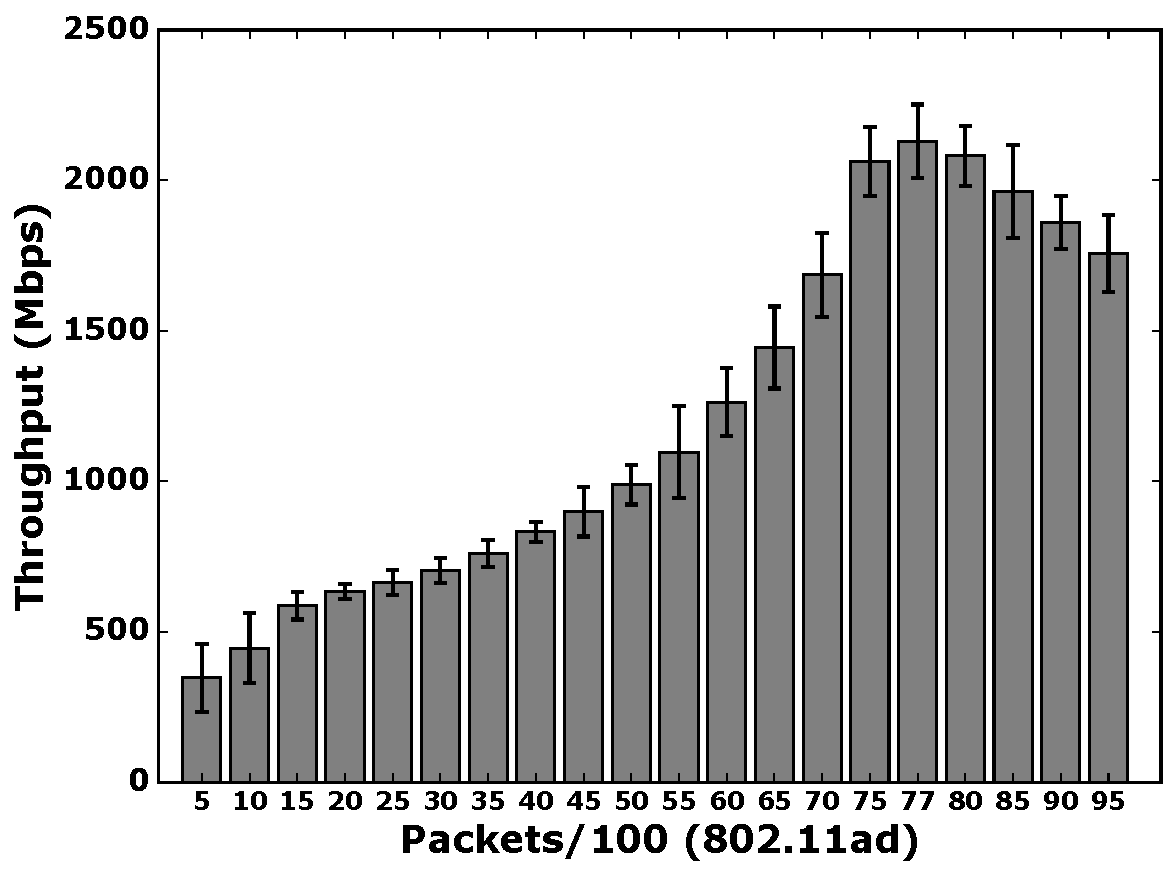
\includegraphics[scale=0.2]{contention/ratio_tput_bar.pdf}
        \label{fig:ratio_tput}
    }\hfill
    \subfigure[Delay (\emph{ofo-queue}) for different $Pkts_{ad}$] {
        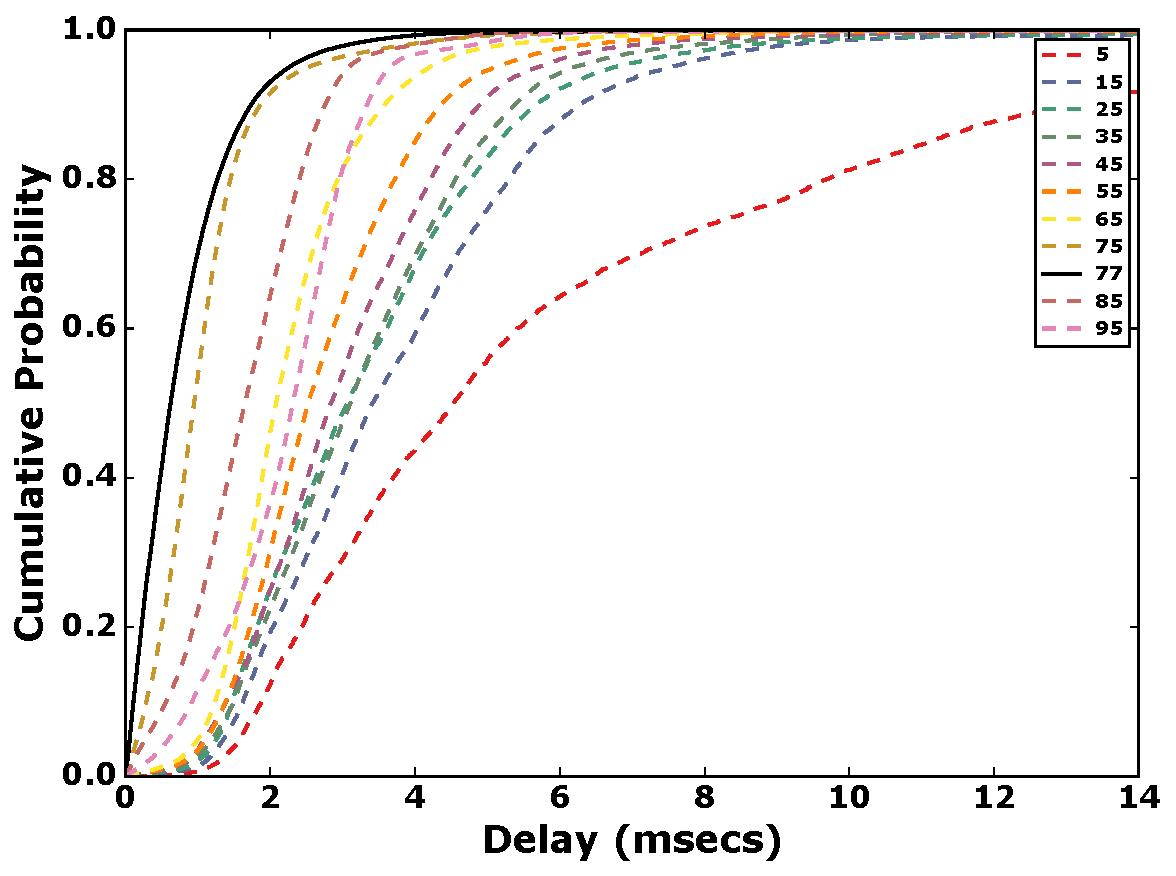
\includegraphics[scale=0.2]{contention/ratio_ofo_delay.pdf}
        \label{fig:ratio_tput_ofo_delay}
    }%\hfill
    %\subfigure[Length of the \emph{ofo-queue} for different $Pkts_{ad}$.] {
    %    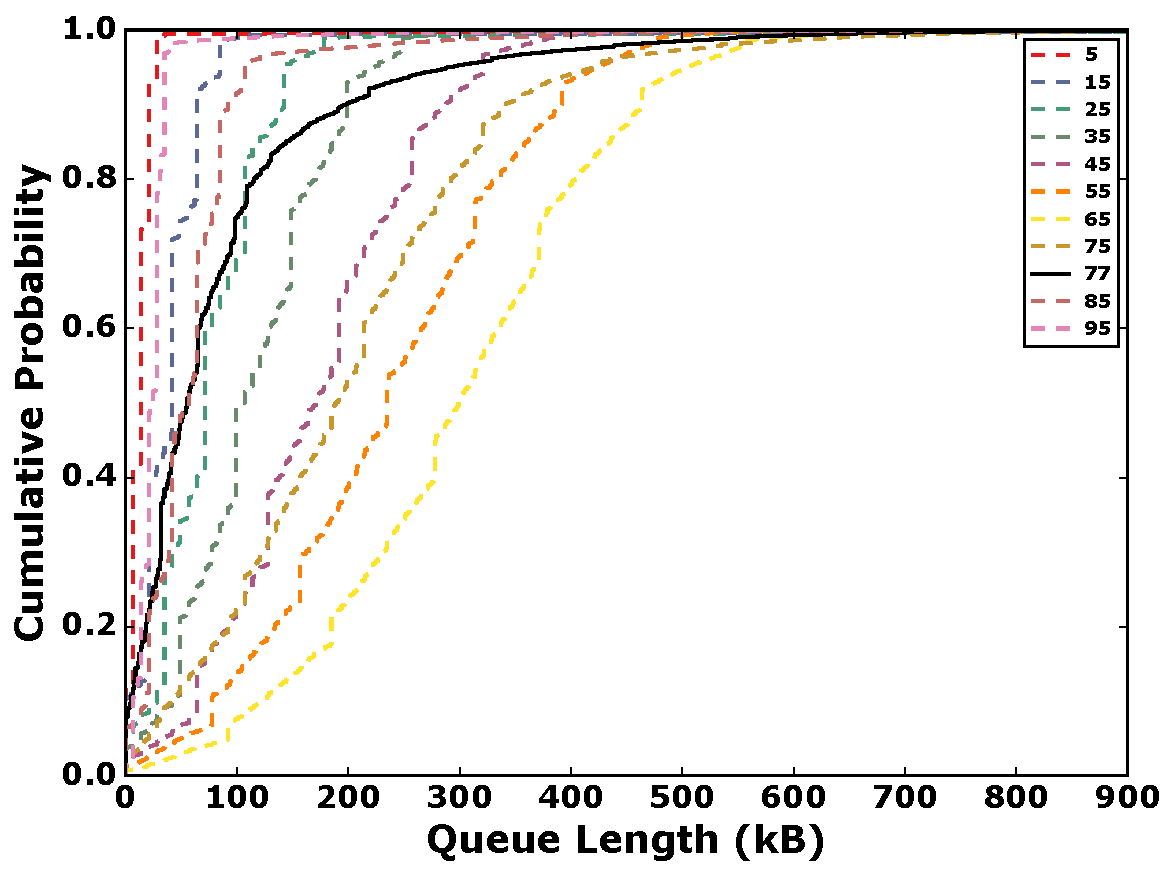
\includegraphics[scale=0.28]{contention/ratio_ofo_q_len.pdf}
    %    \label{fig:ratio_tput_ofo_len}
    %}
    \caption{Impact of packet scheduling decisions.}
\end{figure}

Fig.~\ref{fig:ratio_tput} plots the MPTCP throughput against the
number of packets assigned to the 802.11ad subflow ($Pkts_{ad}$) out
of every 100 packets. We vary $Pkts_{ad}$ between 5 to 95 (with a step
of 5) to cover the entire range of possible assignment ratios. In each
case, the remaining packets (out of 100) are assigned to the 802.11ac
subflow ($Pkts_{ac}=100-Pkts_{ad}$). Maximum throughput of $\sim$2.1
Gbps is achieved with $Pkts_{ad}=77$ and performance worsens as we
move away from this value with the worst throughput being as low as
400 Mbps ($Pkts_{ad}=5$).

We found that the stark difference in performance with different
assignment ratios is a result of the degree to which packets arrive
\textit{out-of-order} in the end-to-end MPTCP flow due to
the specific distribution of traffic among the subflows.
A higher number of out-of-order packets can cause
packets to be buffered in the receiver's \emph{ofo-queue} and in
extreme cases can even result in throttling of the sender because of
limited/no space in the receiver's buffer. In fact, in
Fig.~\ref{fig:ratio_tput_ofo_delay}, which plots the CDF of the delay
experienced by bytes in the \emph{ofo-queue}, we observe that
the $Pkts_{ad}=77$ value (that results in highest throughput) indeed
yields the lowest delay. Moreover, we observe that in general the
$Pkts_{ad}$ values that result in high delay are the ones that result
in lower throughput and vice-versa. 
\if 0
We also plot the CDF of the
occupancy of the \emph{ofo-queue} under different $Pkts_{ad}$
values in fig. \ref{fig:ratio_tput_ofo_len}. Here, one might expect to
see a similar behavior as the delay where the queue lengths are smaller
(indicating less out-of-ordering) for packet assignments that yield
higher throughputs. However, under extreme $Pkts_{ad}$ values
(e.g, 5, 95), the traffic distribution is so skewed towards one of
the subflows that almost all the packets flow through one of
the interfaces, thereby significantly reducing the chance of having an
in-sequence packet being delayed over the other interface. As a result
extreme $Pkts_{ad}$ values (5, 95, 15, 85 15), although sub-optimal
throughput-wise, have queue lengths smaller than the one of the $Pkts_{ad}=77$ case.
Excluding the extremes, other $Pkts_{ad}$ values show a general trend of
having larger queues in conjunction with lower throughputs values.
\fi
\noindent\textbf{Throughput-optimal ratio.} The reason $Pkts_{ad}=77$ results in optimal throughput is that
the underlying packet-distribution ratio imposed by this assignment
$Pkts_{ratio}=Pkts_{ac}/Pkts_{ad}=23/77=0.29$ is nearly identical to
the ratio of the actual individual throughputs of the two interfaces
$Tput_{ratio}=Tput_{ac}/Tput_{ad}=500/1600=0.31$. Assigning packets in
this very specific ratio minimizes the chance of packets arriving
out-of-order at the meta-level MPTCP buffers/queues. Note that
although in-order delivery of packets within a subflow (intra-subflow)
is guaranteed because of SPTCP operation at the subflow level,
global in-order delivery among all subflows (inter-flow) needs
to be achieved through re-ordering at the meta-level.


\section{Performance Issues}
We now look at more challenging scenarios where we show that the 
default MPTCP architecture is unable to adapt, resulting in sub-optimal 
performance which is often worse than that of SPTCP over the
faster subflow.

\begin{figure*}[h]
    \centering
    \subfigure[Network scan: Throughput timeline] {
        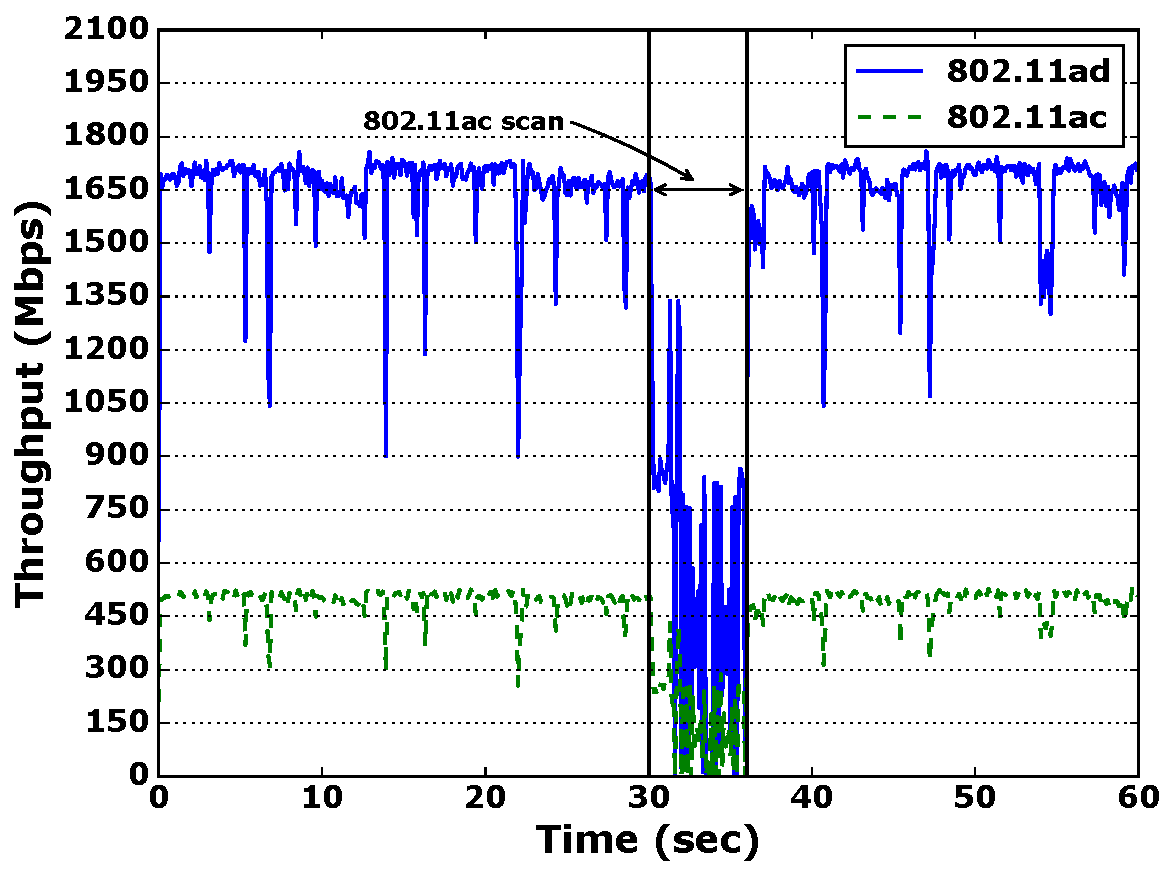
\includegraphics[scale=0.27]{NetworkManagerScan/timeline_no_fix.pdf}
        \label{fig:scan_issue}
    }\hfill
    \subfigure[802.11ac contention: Timeline showing throughput drop during contention] {
        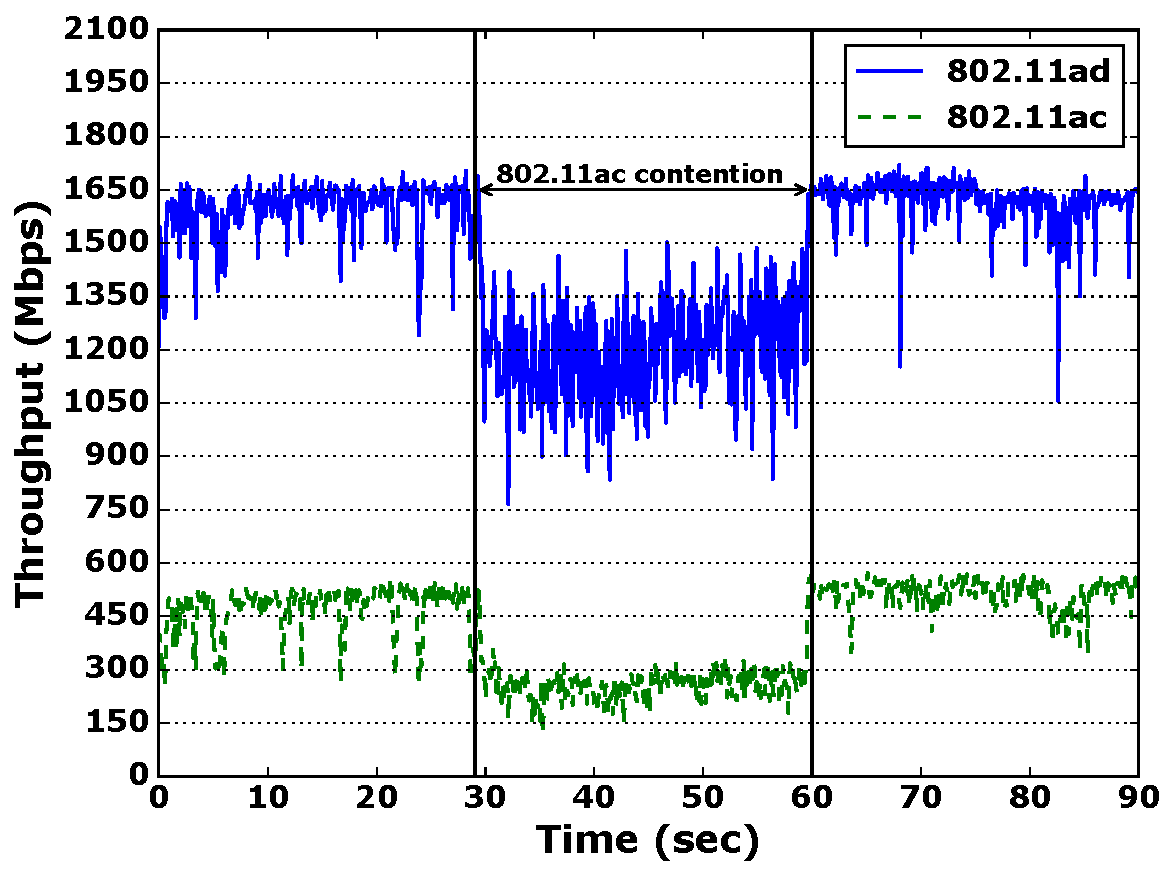
\includegraphics[scale=0.27]{contention/timeline.pdf}
        \label{fig:contention_timeline}
    }\hfill
    \subfigure[802.11ad blockage: 802.11ad throughput drop after re-connection] {
        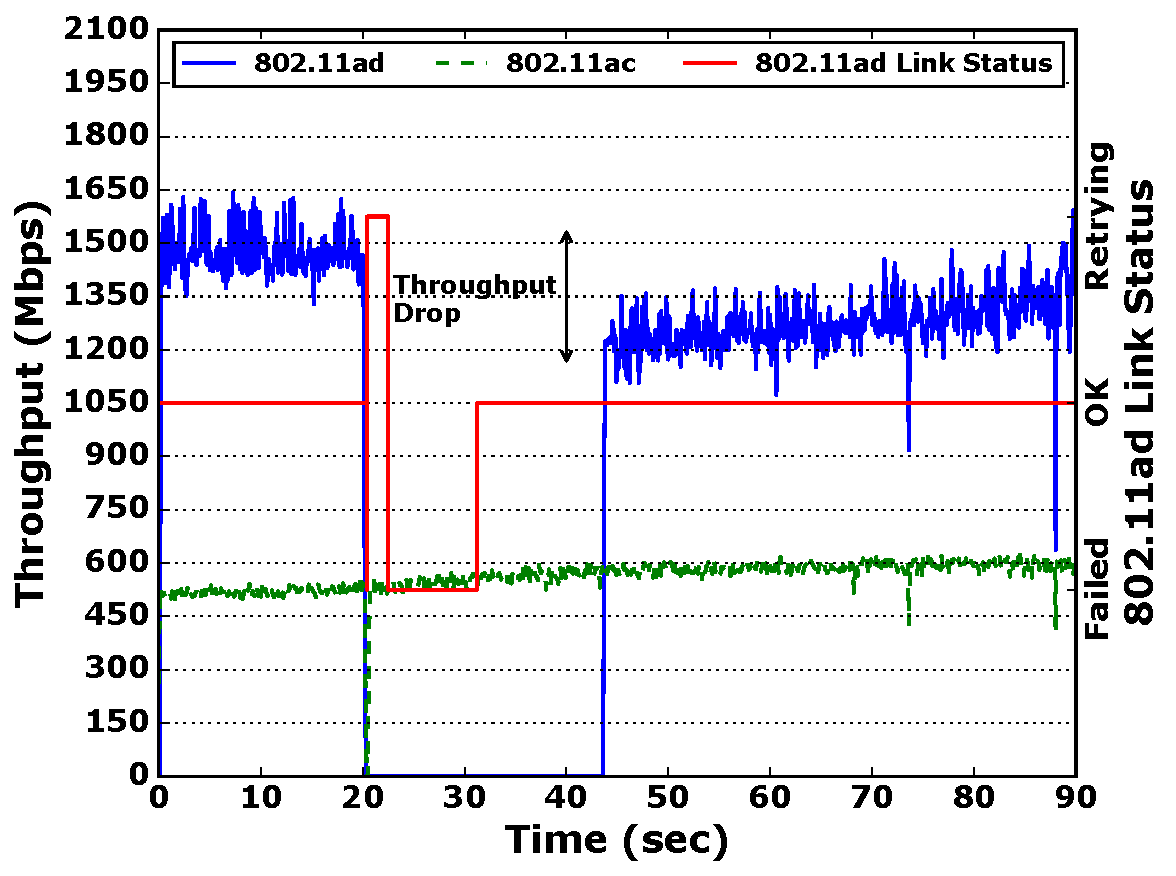
\includegraphics[scale=0.27]{blockage/blockage_tput_drop.pdf}
        \label{fig:blockage_tput_drop}
    }
    \vspace{-0.15in}
    \caption{Performance issues}
    \vspace{-0.1in}
\end{figure*}

\noindent\textbf{Network Scans. }Fig.~\ref{fig:scan_issue} shows the throughput of 802.11ad
and 802.11ac subflows over 60 s and the scan initiated at the 30 s mark. The 802.11ac throughput 
is cut down severely during the scan period (marked as "802.11ac scan") that lasts for 
around 6 s. This is an expected effect of the network scan as the radio is unable to
transmit regular data frames during this period. However, we observe that the 802.11ad 
flow is also impacted negatively during this period, even though the scan takes place in the 
5 GHz band. On investigation, we observed a 6x increase in the amount of data held in 
the \emph{ofo-queue} at the receiver end. During the scan period, the packet
scheduler, which is not aware of the sudden reduction in 802.11ac channel capacity, assigns 
packets in the same ratio as before the scan. This is problematic as the receiver's packet stream now has
\textit{gaps} (missing in-sequence packets) due to stuck 802.11ac packets; these gaps are 
preventing the receiver from delivering packets to the application until the missing packets arrive
or are re-transmitted over the 802.11ad interface.

\noindent\textbf{WiFi (802.11ac) Contention. } Fig.~\ref{fig:contention_timeline} shows a timeline of the
per-flow throughput of a 180 s MPTCP session. We start with a static link where 802.11ad and 802.11ac are 
at their maximum throughputs of $\sim$550 Mbps and $\sim$1650 Mbps, respectively, and we introduce
contention with 300 Mbps TCP cross-traffic at the 30th second for 30 s. The throughput of the 
802.11ac subflow drops by 300 Mbps to around 250 Mbps, as expected. Surprisingly, the 802.11ad subflow is also
affected negatively during the contention period with its throughput dropping below 1200 Mbps and experiencing more variability
than in the interval preceding the start of the contention period. In fact, the MPTCP throughput during the 
contention period averages to $\sim$1450(=1200+250) Mbps, which is less than even that of 802.11ad
operating alone (1650 Mbps). Note that 802.11ad channel capacity is unchanged as the contention is introduced 
only on the 802.11ac's operating channel. On further investigation, we found that during the
contention period the receiver advertised buffer space (\emph{recv\_win}) reduces significantly. 
Remember that the \emph{recv\_win} is maintained at the meta-level and, although
advertised on both subflows, is actually shared among them. Under such a scenario, the meta-level global sequence numbers
cannot advance, even though \emph{cwnd} allows for it, since the
meta-level buffers at the receiver are full, resulting in reduction of
throughput on both interfaces.

\noindent\textbf{60 GHz (802.11ad) Blockage. } Fig. \ref{fig:blockage_tput_drop} shows a
timeline of subflow throughputs along with link status {\tt Failed/OK/Retrying} as reported by 
the 802.11ad driver. The blockage is introduced at the $20^{th}$ second causing the link status 
to switch to fail after a further 2 s. Once the blockage is removed, connection at the MAC layer is
restored at the $30^{th}$ second. We observe the following two issues:
\\
(i) Although the 802.11ad link is restored at the $30^{th}$ second, MPTCP does not resume traffic 
on the 802.11ad subflow for another $\sim$20 seconds until the $49^{th}$ second. We found that
In the case of a timeout-based loss event, TCP congestion-control sets the {\tt pf} flag on the socket,
indicating the flow to be \emph{potentially failed}. The MPTCP scheduler treats subflows with 
the {\tt pf} flag set as being unavailable and does not schedule any packets on them. TCP
congestion-control, on the other hand, is waiting for an ACK to unset
the {\tt pf} flag and enter the {\tt TCP\_CA\_RECOVERY} state that can
restore the \emph{cwnd} to the value before the loss event. Since no
packets are being directed to the 802.11ad subflow, only a subflow-level re-transmission 
of the 802.11ad subflow can trigger the transmission of an ACK on the receiver side. However, 
multiple timeout-based losses during the blockage period can lead to excessively 
high retransmission timeouts, and consequently to long delays before an ACK is received.
\\
(ii) On resumption, 802.11ad flow starts with a \emph{cwnd} and
\emph{ssthresh} that are half of their pre-loss values. Fig. \ref{fig:blockage_tput_drop} shows 
a sample timeline where the 802.11ad flow resumes to 1350 Mbps instead of 1650 Mbps. Note that
this behavior depends on the exact specifics of the TCP congestion-control state at the time 
it enters the recovery state. Nonetheless, we observed this quite often and it does have a
non-negligible impact on throughput.

\begin{figure*}[ht]
    \centering
    \subfigure[Network Scan (Timeline)] {
        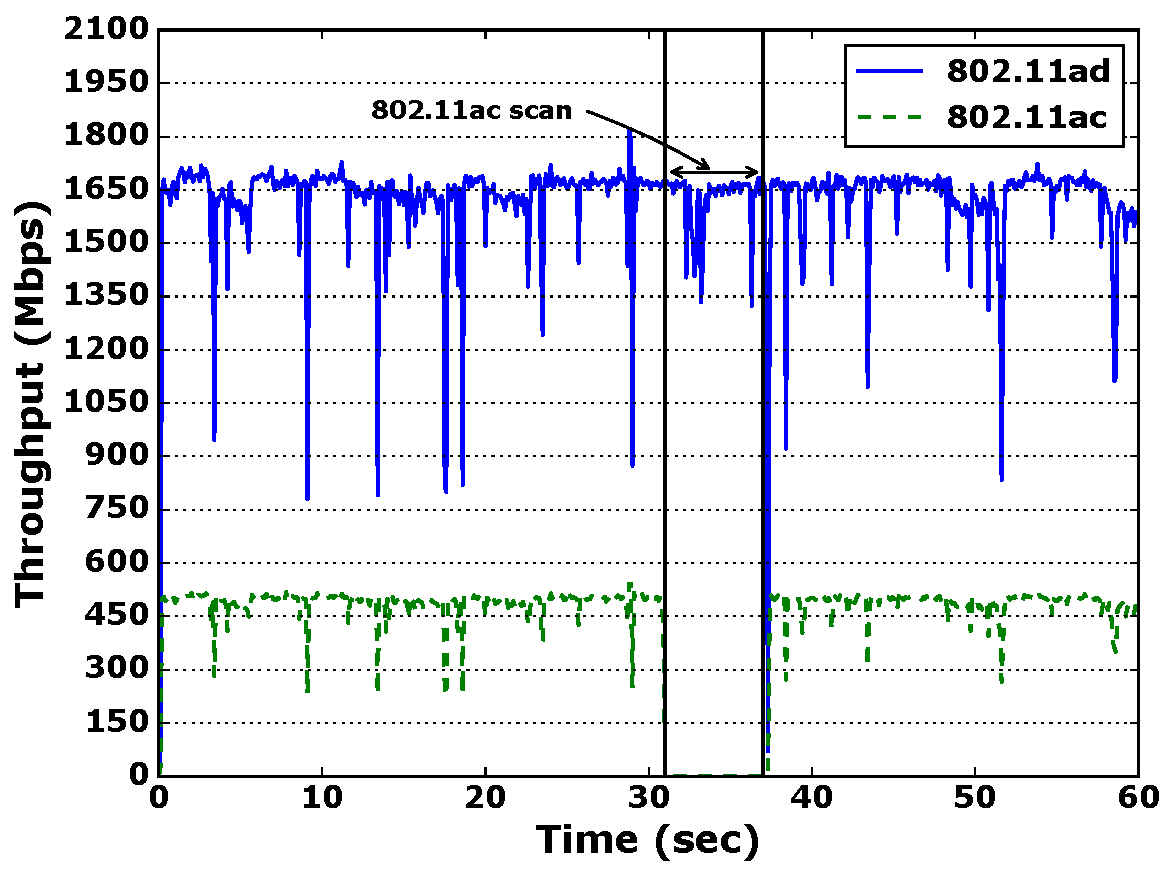
\includegraphics[scale=0.27]{NetworkManagerScan/timeline_fix.pdf}
        \label{fig:scan_fixed}
    }\hfill
    \subfigure[\emph{minRTT} vs. \emph{FixedRatio}] {
        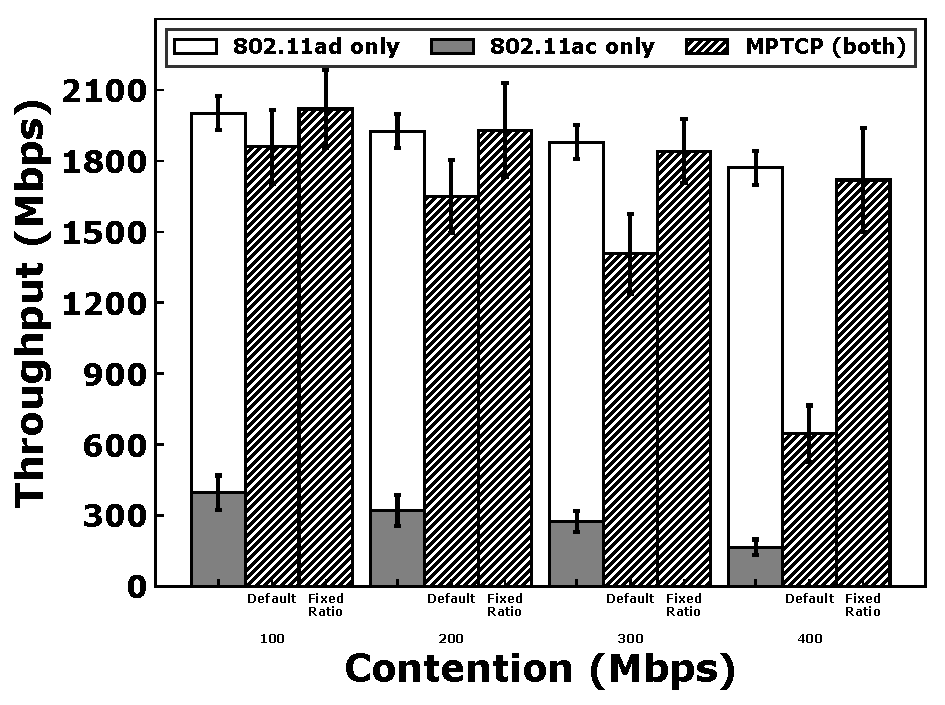
\includegraphics[scale=0.34]{contention/barplot.pdf}
        \label{fig:contention_barplot}
    }\hfill
    \subfigure[802.11ad Blockage: Improved recovery time] {
        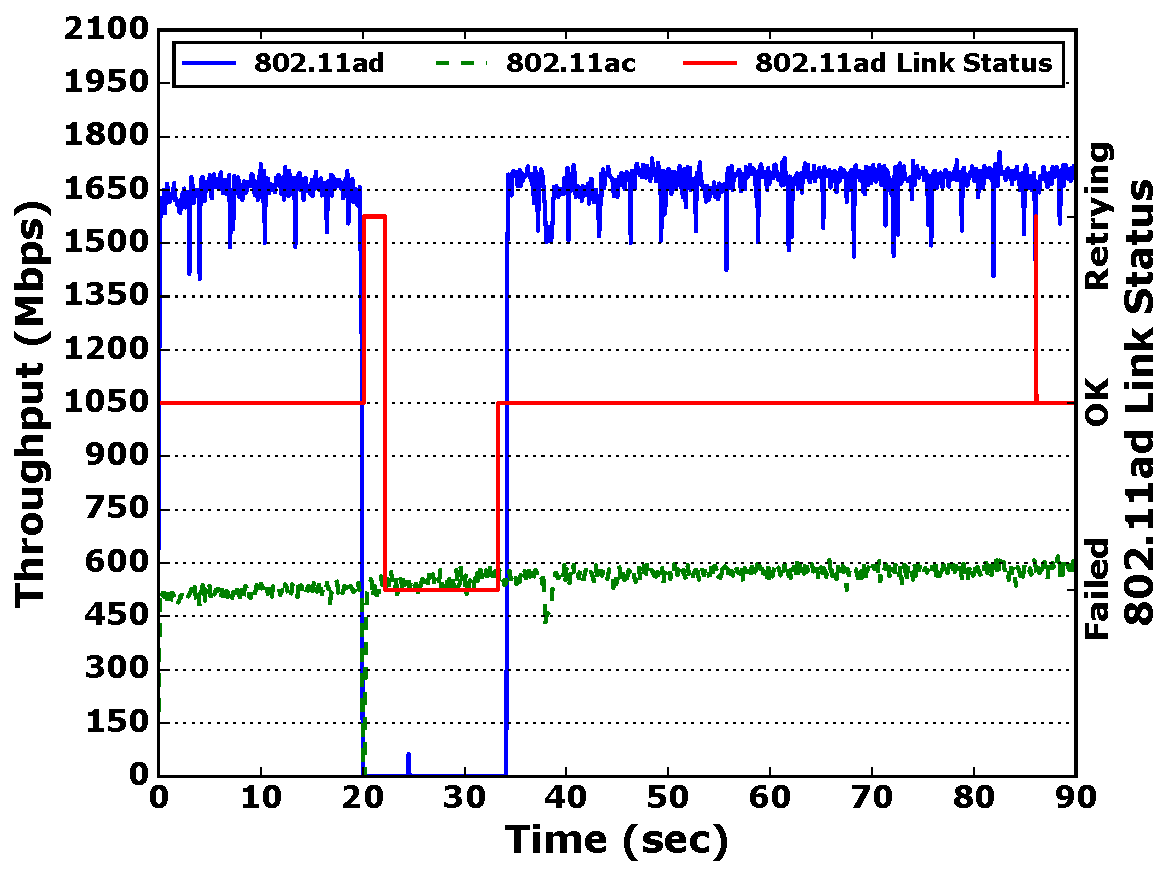
\includegraphics[scale=0.27]{blockage/blockage_fixed.pdf}
        \label{fig:blockage_recovery}
    }
    \vspace{-0.15in}
    \caption{\name}
    \vspace{-0.1in}
\end{figure*}



\bibliographystyle{ACM-Reference-Format}
\bibliography{references}

\end{document}
